%%%%%%%%%%%%%%%%%%%%%%%%%%%%%%%%%%%%%%%%%%%%%%%%%%%%%%%%%%%%%%%%%
\begin{frame}[fragile]
\frametitle{\textbf{\textcolor{orange}{Taylor shift by $a$}}}

\begin{Definition}
The \textcolor{red}{\textbf{Taylor shift by $a$}} of a polynomial $P\in R[x]$, with $R$ a field (e.g., $\mathbb{Z}$) consists of evaluating the coefficients of $P(x+a)$.
\end{Definition}

So, for a polynomial $P=\sum_{0\leq i \leq n} f_i\,x^i\, \in \, \mathbb{Z}[x]$ and $a\in\mathbb{Z}$, we want to compute the coefficients $g_0$,...,$g_n\,\in\,\mathbb{Z}$ of the Taylor expansion :

$$\textcolor{darkgreen}{Q(x)=\sum_{0\leq k \leq n}g_k\, x^k=P(x+a)=\sum_{0\leq i \leq n}f_i\, (x+a)^i}$$ 

There are several methods to compute this, the classical ones deal with the \textit{Horner's method}. There are also asymptotically fast methods, and in particular \textcolor{red}{\textit{Divide \& Conquer method (D{\&}C)}} which we will use.

\end{frame}
%%%%%%%%%%%%%%%%%%%%%%%%%%%%%%%%%%%%%%%%%%%%%%%%%%%%%%%%%%%%%%%%%

%%%%%%%%%%%%%%%%%%%%%%%%%%%%%%%%%%%%%%%%%%%%%%%%%%%%%%%%%%%%%%%%%
\begin{frame}[fragile]
\frametitle{\textbf{\textcolor{orange}{Divide \& Conquer method (D{\&}C)}}}

\begin{Definition}
The \textcolor{violet}{\textbf{size of a polynomial}} of degree $d$ is $d+1$.
\end{Definition}

\textcolor{darkgreen}{\textbf{size of the polynomials considered :}} $n = 2^e$ (so degree : $d = 2^e - 1$)

\begin{block}{}
\textcolor{blue}{\textbf{The Divide \& Conquer method consists of :}}

\begin{enumerate}
\item \textcolor{violet}{split} the polynomial as : $P(x) = P^{(0)}(x+1)+(x+1)^{n/2}\times P^{(1)}(x+1)$
\item \textcolor{violet}{evaluate} $P^{(0)}(x+1)$ and $P^{(1)}(x+1)$ \textcolor{violet}{recursively}
\item \textcolor{violet}{compute a product} when $P^{(1)}(x+1)$ is evaluated
\item \textcolor{violet}{compute a sum} when $P^{(0)}(x+1)$ and the product are evaluated
\end{enumerate}
\end{block}

These are the four main things to implement to realize the \textit{Taylor shift by $1$}.

\end{frame}

%%%%%%%%%%%%%%%%%%%%%%%%%%%%%%%%%%%%%%%%%%%%%%%%%%%%%%%%%%%%%%%%%

%%%%%%%%%%%%%%%%%%%%%%%%%%%%%%%%%%%%%%%%%%%%%%%%%%%%%%%%%%%%%%%%%
\begin{frame}[fragile]
\frametitle{\textbf{\textcolor{orange}{D{\&}C tree for $n=8=2^3$}}}

\begin{center}
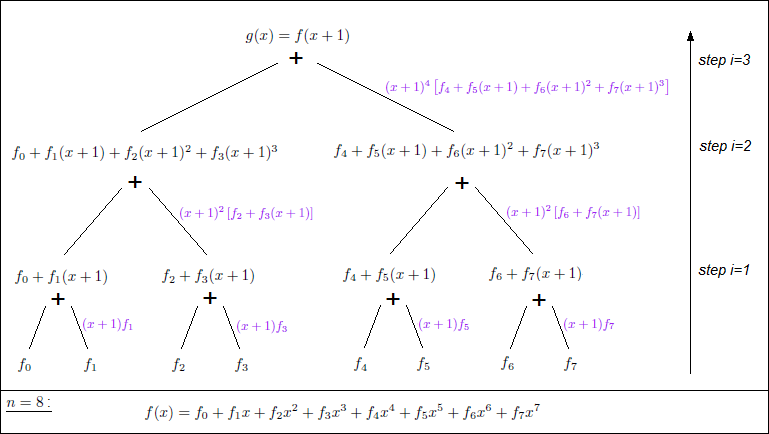
\includegraphics[scale = 0.37]{ComputingTree.png}\\
\textbf{D{\&}C computing tree}
\end{center}

\begin{block}{}
In parallel, we consider the tree by levels (from its base) and not recursively.
\end{block}
.
\end{frame}

%%%%%%%%%%%%%%%%%%%%%%%%%%%%%%%%%%%%%%%%%%%%%%%%%%%%%%%%%%%%%%%%%

%%%%%%%%%%%%%%%%%%%%%%%%%%%%%%%%%%%%%%%%%%%%%%%%%%%%%%%%%%%%%%%%%
\begin{frame}[fragile]
\frametitle{\textbf{\textcolor{orange}{Compute the $(x+1)^{2^i}$s}}}

For multiplication, we need to compute the polynomials \textcolor{red}{$(x+1)^{2^i}$} for $i\in \mbox{\textlbrackdbl} 0, e-1\mbox{\textrbrackdbl}$.\\
\vspace{4mm}
\begin{cb}
According to the binomial theorem, we have in general :
$$\textcolor{darkgreen}{\forall n\in \mathbb{N},\, (x+1)^n = \sum_{k=0}^{n} {n \choose k}\, x^k \mbox{ with } {n \choose k} = \cfrac{n!}{k!\, (n-k)!}}$$
\end{cb}

\textcolor{blue}{\textbf{Consequence :}} we need to compute the sequence $(i!)_{0 \leq i \leq n}$.

\end{frame}

%%%%%%%%%%%%%%%%%%%%%%%%%%%%%%%%%%%%%%%%%%%%%%%%%%%%%%%%%%%%%%%%%

%%%%%%%%%%%%%%%%%%%%%%%%%%%%%%%%%%%%%%%%%%%%%%%%%%%%%%%%%%%%%%%%%
\begin{frame}[fragile]
\frametitle{\textbf{\textcolor{orange}{Factorial sequence}}}

\begin{block}{}
We compute only the sequence \textcolor{red}{$(i!)_{1 \leq i \leq n}$} (power of $2$).

\textit{\textcolor{darkgreen}{Notation :}} $a \underline{\bf{\times}} b = \prod_{k=a}^{b} k$ (e.g. $9 \underline{\bf{\times}} 13 = 9 \times 10 \times 11 \times 12 \times 13$).
\end{block}

\begin{center}
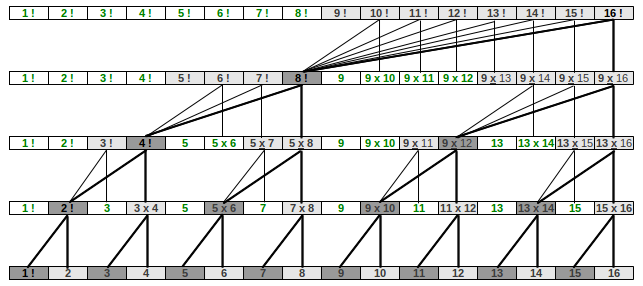
\includegraphics[scale = 0.273]{facto.png}\\
\textbf{Mapping of the computation of the sequence $(i!)_{1 \leq i \leq 16}$}
\end{center}

$n/2$ threads do products using a ``pillar'' factor (in the darkest boxes).\\
\textcolor{blue}{\textbf{Work :}} $\Theta(n\,log(n))$

\end{frame}

%%%%%%%%%%%%%%%%%%%%%%%%%%%%%%%%%%%%%%%%%%%%%%%%%%%%%%%%%%%%%%%%%

%%%%%%%%%%%%%%%%%%%%%%%%%%%%%%%%%%%%%%%%%%%%%%%%%%%%%%%%%%%%%%%%%
%\begin{frame}[fragile]
%\frametitle{\textbf{\textcolor{orange}{Factorial sequence}}}

%\begin{verbatim}
%__global__ void create_factorial_stepi_GPU(sfixn *Fact, sfixn n, \
%                           sfixn e, sfixn p, double pinv, sfixn L){
%  sfixn k = blockIdx.x * blockDim.x + threadIdx.x;
%  sfixn j, part, pos, base;
%  sfixn B = 2 * L;
%
%  if (k < n/2){
%      part = k / L;
%      pos = k % L;
%      j = L + part*B + pos;
%      base = Fact[L + part*B - 1];
%      Fact[j] = mul_mod(base, Fact[j], p, pinv);
%}}
%\end{verbatim}

%\begin{center}
%\textbf{Procedure showing a step of computation}
%\end{center}
%\end{frame}

%%%%%%%%%%%%%%%%%%%%%%%%%%%%%%%%%%%%%%%%%%%%%%%%%%%%%%%%%%%%%%%%%

%%%%%%%%%%%%%%%%%%%%%%%%%%%%%%%%%%%%%%%%%%%%%%%%%%%%%%%%%%%%%%%%%
\begin{frame}[fragile]
\frametitle{\textbf{\textcolor{orange}{Store the $(x+1)^{2^i}$s}}}

\begin{center}
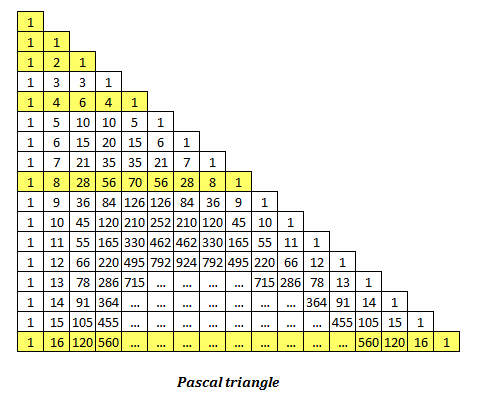
\includegraphics[scale = 0.364]{PascalTriangle.png}
\end{center}

\textcolor{darkgreen}{\textbf{Array \textit{Monomial\_shift\_device} for $n = 16 = 2^4$ :}}
\begin{center}
\tiny{
\begin{tabular}{|c||c||c|c||c|c|c|c||c|c|c|c|c|c|c|c|} \hline
1 & 1 & 2 & 1 & 4 & 6 & 4 & 1 & 8 & 28 & 56 & 70 & 56 & 28 & 8 & 1 \\ \hline
\end{tabular}
}
\end{center}

\textbf{At step $i$, $local\_n = 2^i$ :}
$$\textcolor{red}{\forall j\in \mbox{\textlbrackdbl} 0, local\_n - 1\mbox{\textrbrackdbl},\; Monomial\_shift[local\_n + j] = {local\_n \choose j + 1}}$$

\end{frame}

%%%%%%%%%%%%%%%%%%%%%%%%%%%%%%%%%%%%%%%%%%%%%%%%%%%%%%%%%%%%%%%%%
